\section{Le Bras Droit du Cruciverbiste (i.e. La Résolution de Mots Croisés)}

La troisième tâche est la résolution d'indices de mots croisés. Le concept est simple et ressemble aux tâches précédentes dans son exploitation du réseau sémantique. Tandis que le chercheur de synonymes calcule la distance entre des mots individuels et le désambiguïseur trouve la distance entre deux séquences de mots, le resolveur de mots-croisés cherche la distance entre une séquence de mots (l'indice) et un mot (le mot cible). Comme précédemment, le noyau du programme est donc une recherche dans la matrice de relations pour trouver un certain nombre de mots candidats. Par contre, des étapes supplémentaires sont nécessaires pour faire en sorte que les mots cibles adhèrent à certaines contraintes imposées par le jeu.

Le principe des mots croisés est de remplir une grille de lettres en fonction d'indices, et en fonction des deux contraintes qui sont la longueur des mots cibles et les caractères qui ont déjà été devinés dans la grille. Notre application est un outil support qui permet de fournir des mots candidats au cruciverbiste\footnote{Un amateur de mots croisés}. A part ces deux contraintes, il est important que les mots candidats correspondent à la catégorie syntaxique indiquée par l'indice. Notons que pour l'instant l'application ne détecte que les mots des catégories \lq{nom}\rq, \lq{adj}\rq, \lq{adv}\rq{} et \lq{verbe}\rq, puisque les autres catégories ne sont pas présentes dans le réseau. Par exemple, pour l'indice \lq{escroqués}\rq, les mots candidats doivent être des participes passés qui sont conjugués au masculin pluriel, et pour l'indice \lq{a l'air chouette}\rq, les mots candidats doivent être des verbes conjugués à la troisème personne singulier du présent indicatif\footnote{Les bonnes réponses sont \lq{eus}\rq{}  et \lq{ulule}\rq{} respectivement}.

Le processus suivi est donc séquentiel et peut être représenté par le schéma suivant:   

\begin{figure}[!ht]
\centering
\def\svgwidth{\columnwidth}
\input{crossword_schema.pdf_tex}
\caption{Le schéma du traitement pour la résolution des indices de mots croisés}
\label{fig:schema_crosswords}
\end{figure}

\subsection{Les étapes de traitement}

\subsubsection{Etape 1 : Identification de la catégorie syntaxique du mot cible}%\label{sec:crossetape1}
Les indices sont de petites séquences de mots qui sont très rarement des phrases complètes et bien formées. Ils correspondent souvent à un syntagme particulier et contiennent parfois des ambiguïtés de catégorie syntaxique dont il faut tenir compte. Il est aussi possible à cette étape d'identifier quelques marques de flexion qui peuvent indiquer la forme du mot cible. Le réseau sémantique ne contient a priori que des lemmes et donc il est important de garder ces indices flexionnels pour re-fléchir les mots candidats à l'étape 3. %(Voir section~\ref{sec:crossetape3).  

Un étiqueteur syntaxique automatique tel que MElt[\hyperref[bib:melt]{~\ref*{bib:melt}}] est peu adapté pour cette identification puisqu'il se base sur les probabilités pour renvoyer la séquence de tags la plus probable pour l'indice. Ceci signifie que le tag prédit peut ne pas correspondre à un des tags possibles pour un mot donné ou les ambiguïtés peuvent ne pas être trouvées. De plus, de tels étiqueteurs sont dépendants de leurs données d'entraînement, et les indices des mots croisés sont d'une forme très différente des données du French TreeBank sur lequel MElt a été entrainé. Nous choisissons donc de faire une analyse point à point des mots de l'indice afin de renvoyer toutes les possibilités catégorielles pour chaque mot. Le Lefff (Lexique des Formes Fléchies du Français)[\hyperref[bib:lefff]{~\ref*{bib:lefff}}] est utilisé pour retrouver toutes les catégories syntaxiques et marques flexionnelles de chaque mot. Cette méthode renvoie évidemment plus de séquences possibles de catégories syntaxiques que souhaitées et crée donc de l'ambiguïté artificielle. Cependant, c'est un moyen d'augmenter le rappel des résultats, même si la précision en souffre. Il est important pour nous de renvoyer le plus de mots candidats possibles et une erreur d'étiquetage syntaxique à cette étape peut significativement nuire les chances de trouver les bons candidats par la suite.

La catégorie syntaxique du mot cible peut être identifiée à partir de la séquence d'ensembles de catégories grâce à la régularité des formes des indices. Si un indice contient un seul mot, les catégories cibles sont celles du mot de l'indice. Sinon, la catégorie dépend en grande partie des premiers mots de l'indice. Par exemple, si un indice commence par un nom, ou une séquence \lq{det nom}\rq{} ou une séquence \lq{det adj nom}\rq{}, la catégorie cible, étant donné qu'il n'y a pas d'ambiguïté catégorielle, serait un nom. Dans certains cas, il est aussi possible d'identifier quel mot de l'indice indique la flexion du mot cible. Cette identification se fait à l'aide d'une mini-grammaire de seulement 18 règles, qui sont reproduites ci-dessous :

\begin{framed}
det nc -\textgreater 2, nc\newline
det adj nc -\textgreater 3, nc\newline
adj nc -\textgreater 2, nc\newline
nc -\textgreater 1, nc\newline
adj prep -\textgreater 1, adj\newline
adv v -\textgreater 2, v\newline
advm v -\textgreater 2, v\newline
advneg v -\textgreater 2, v\newline
advneg advneg v -\textgreater 3, v\newline
v -\textgreater 1, v\newline
clr v -\textgreater 2, v\newline
prel v -\textgreater 2, adj \newline
cln v -\textgreater 2, n\newline
prep nc -\textgreater ?, adv\newline
ce v det nc -\textgreater 4, nc\newline
adj coo adj -\textgreater 1, adj\newline
nc coo nc -\textgreater 1, adj\newline
pri v -\textgreater 2, adj
\end{framed}

Chaque ligne représente une règle différente. A gauche de la flèche est la séquence de mots qui indique, au début d'un indice, une certaine catégorie syntaxique pour le mot cible. A droite de la flèche est l'indice (à partir de 1) du mot de la partie gauche dont les informations grammaticales seront utilisées pour fléchir les mots cibles (qui seront des lemmes), suivi de la catégorie syntaxique du mot cible. Dans le cas où aucun mot de l'indice en particulier donne des indices flexionnels, \lq{?}\rq{} indique que les indices flexionnels sont inconnus. Par exemple, un indice tel que \lq{avec soin}\rq{} correspond à la règle \lq{prep nc -\textgreater ?, adj}\rq{}, où la catégorie cible serait \lq{adv}\rq{}, mais où aucun mot entre la préposition et le nom fournit d'indice flexionnels.

Le jeu d'étiquettes utilisées est celle du Lefff\footnote{Ce jeu a été réduit pour ne contenir que les noms, adjectifs, adverbes et verbes et les catégories nécessaire pour la mini-grammaire}, qui est utilisé pour retrouver les formes fléchies. Un même indice peut correspondre à plusieurs règles différentes si un mot donné est ambigu pour la catégorie syntaxique.

Les catégories syntaxiques sont retenues pour le parcours du réseau et les informations grammaticales pour retrouver les formes fléchies correspondant aux lemmes trouvés dans le réseau.

Remarque : Une particularité des indices est que parfois elles peuvent contenir plusieurs parties, séparées d'une virgule et qui représentent plusieurs sous-indices à l'intérieur de l'indice. Par exemple, un indice peut avoir la forme \lq{habillée, fringuée}\rq{} et dans ce cas, il est souhaitable de séparer cet indice en \lq{habillée}\rq{} et \lq{fringuée}\rq{} afin d'avoir la meilleure chance de trouver la catégorie voulue. Idéalement, ces deux parties devraient aussi correspondre en termes de catégorie syntaxique, ce qui signifie qu'il faudrait en théorie ne garder que les catégories cibles qui correspondent aux deux parties de l'indice. Par contre, nous optons pour le choix de garder toutes les catégories potentielles à partir des deux parties de l'indice pour nous assurer de la couverture maximale. 

\subsubsection{Etape 2 : Recherche dans le graphe}%\label{sec:crossetape2}

Une fois que la catégorie syntaxique de la solution est ciblée (ou au moins 
réduite à une liste de catégories possibles), et les mots de l'indice sont 
lemmatisés, il est possible d'utiliser le réseau sémantique pour trouver les 
mots les plus proches à l'indice. Ici nous testons la première stratégie de 
recherche dans le graphe: l'algorithme de parcours en largeur pour renvoyer les 
k plus proches voisins de chaque lemme. Une extension serait d'implémenter aussi 
la recherche de la matrice complète. Le choix des plus proches candidats va 
dépendre de l'algorithme utilisé.

Un indice peut contenir plusieurs lemmes et avec le réseau sémantique, il est facile de renvoyer les voisins (avec leurs distances) d'un mot individuel. Pour le parcours en largeur il s'agit de parcourir le graphe jusquà'ce que les k plus proches voisins sont trouvés. Dans la matrice complète il est possible d'atteindre la liste complète des sommets du réseau avec leurs distances du mot recherché. 

Les voisins d'un lemme donné peuvent être vu comme un vecteur où les paramètres sont les voisins et les valeurs sont leurs distances du lemme. Par exemple un indice \lq{lemme1 lemme2 lemme3}\rq{} aurait trois vecteurs différents pour représenter chacun des lemmes, chacun avec un certain nombre de paramètres spécifiés (en fonction de l'algorithme de recherche utilisé), qui ne seront pas forcément les mêmes pour chaque vecteur (si seulement les k plus proches sont trouvés):

\begin{framed}
vec\_lemme1 : \textless{a: 1, b: 2, c: 3}\textgreater \newline
vec\_lemme2 : \textless{a: 1, b: 5, d: 4}\textgreater \newline
vec\_lemme3 : \textless{a: 4, c: 1, e: 1}\textgreater 
\end{framed}

Le vecteur global doit être représentatif des trois lemmes et des paramètres que contiennent leurs vecteurs. Si la matrice complète est utilisée, les vecteurs des lemmes contiendraient les mêmes voisins est un moyennage des distances est possible pour chaque voisin. Par contre, un moyennage simple des valeurs n'est pas possible pour le parcours en largeur, puisque les voisins non-représentés auraient une valeur infinie pour la distance, ce qui fausserait les distances moyennées. Le choix dans ce cas-là est donc d'ajouter les vecteurs pour en faire un vecteur global, et dans le cas où un paramètre apparaît dans plusieurs vecteurs, comme ci-dessus avec \lq{a}\rq{}, \lq{b}\rq{} et \lq{c}\rq{}, la distance minimale est choisie. Les trois vecteurs ci-dessus aurait alors comme vecteur global:

\begin{framed}
vec\_indice : \textless{a: 1, b: 2, c: 1, d: 4, e: 1}\textgreater 
\end{framed}

Remarques sur les formes recherchées : les lemmes des mots de l'indice sont recherchés dans le réseau, suffixés de leurs catégories syntaxiques possibles, ce qui signfie qu'un mot qui est syntaxiquement ambigu sera recherché plusieurs fois. Si le lemme ne se trouve pas dans le Lefff, au lieu d'abandonner la recherche de ce mot, nous utilisons le mot-forme par défaut, en espérant que ce mot appartient au réseau (particulièrement important pour les noms propres par exemple).\footnote{Même si le réseau ne devraient pas contenir de formes fléchies, il est possible qu'il en contient à cause des erreurs de tagging, et donc nous exploitons cette faiblesse ici pour augmenter la chance de retrouver le plus de mots de l'indice possibles.}. Les catégories syntaxiques cibles sont celles obtenues à partir de la mini-grammaire est en cas de non-identification de catégorie, des candidats de toute catégorie seront recherchés.

\subsubsection{Etape 3 : Conjugaison des lemmes obtenus}%\label{sec:crossetape3}

Les résultats de la recherche du graphe sont (pour la plupart) des lemmes, qui
sont à modifier pour correspondre à la forme du mot recherché. En utilisant 
l'ensemble de catégories et d'informations grammaticales obtenues lors de 
l'étape 1, cette étape cherche les formes fléchies correspondant à chaque 
lemme et vérifie lesquelles correspondent aux informations grammaticales 
recherchées pour les mots candidats.

La ressource utilisée est encore une fois le Lefff, avec pour chaque lemme qui y apparaît, ces catégories syntaxiques possibles et les formes fléchies associées. En connaissant les catégories syntaxiques possibles pour le mot cible (obtenues à l'étape 1), les formes fléchies du lemme sont triées en fonction de leur correspondance aux informations grammaticales aussi obtenues à l'étape 1. Si un trait grammatical (ex: 'nombre') est exprimé pour les flexions voulues, la forme fléchie sera retenue seulement si elle a la même valeur de trait (pourvu que ce trait soit exprimé).

Par exemple, si l'indice est \lq{mangée}\rq{}, les informations grammaticales retenues sont que la catégorie est un participe passé et que le mot recherché doit être féminin singulier. Les voisins du lemme \lq{manger}\rq{} seront recherchés dans le réseau et renvoyés:

\begin{framed}
consommer, alimenter, boire etc.
\end{framed}

Il existe un grand nombre de formes fléchies de ces verbes, mais dont un petit nombre correspondent aux contraintes grammaticales \lq{féminin singulier}\rq{}. Les formes suivantes seront alors rejetées:

\begin{framed}
consommâtes, consommèrent, consommé, consomme, ..., alimentez, alimentées, etc.
\end{framed}

et les formes suivantes retenues:

\begin{framed}
consommée, alimentée, bue
\end{framed}

\subsubsection{Etape 4 : Filtrage selon les contraintes}%\label{sec:crossetape4}

La dernière étape filtre les candidats fléchis afin de ne renvoyer que les candidats qui se conforment aux contraintes de longueur de mot et de caractères déjà devinés. Il n'est pas possible de faire cette étape avant la conjugaison, puisque la conjugaison des lemmes peut avoir pour effet un changement dans la longueur du mot et des caractères qui y apparaîssent.

Souvent dans les outils d'aide de résolution de mots fléchés, cette étape est la seule incluse dans le programme, et donc un grand nombre de mots correspondent aux contraintes de longueur et de caractères. Dans notre programme, cette étape sert à enlever la grande quantité de bruit dans les résultats produits directement à partir du réseau, et permet de raffiner en grande partie les résultats. L'avantage d'utiliser le réseau est qu'il y a plus de chance d'avoir des résultats qui correspondent à l'indice donné et non pas des mots candidats indépendant de l'indice, ce qui permet un traitement plus sophistiqué à cette étape.

\subsection{L'interface graphique}

L'interface graphique, implementée en python en utilisant les bibliothèques 
Tkinter et PMW sert à visualiser les résultats renvoyés aux différentes 
étapes du processus. Elle est mi-chemin entre un outil pour un joueur de mots 
croisés, qui ne s'intéresse qu'aux mots qui se conforment aux contraintes 
données et un outil plus pédagogue pour montrer les étapes du traitement.

\begin{center}
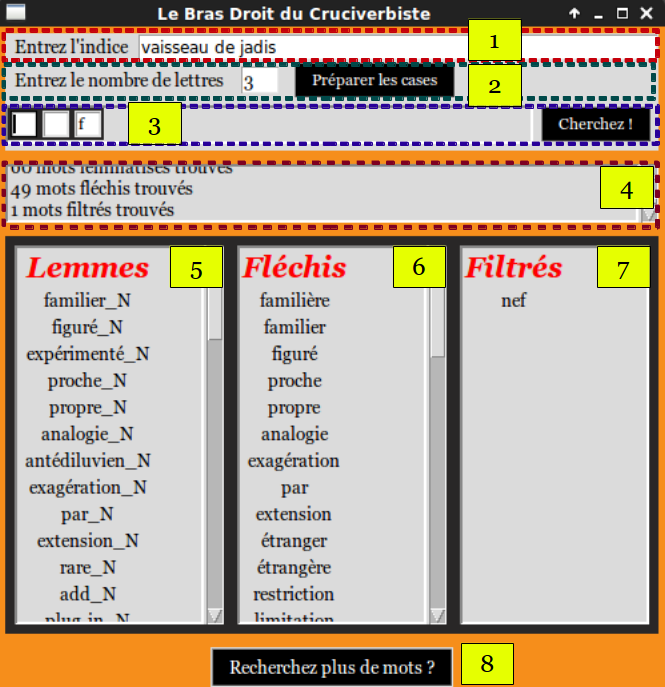
\includegraphics{CrossWordInterface.png}
\end{center}

\begin{enumerate}
    \item{L'indice qui sert à deviner le mot recherché}
    \item{Le nombre de lettres du mot recherché. En cliquant sur \lq{Préparer les cases}\rq, cette contrainte sera enregistrée et les cases générées en 3.}
    \item{Les cases pour entrer les caractères déjà devinés. Cette contrainte sera prise en compte dans le filtrage des mots candidats}
    \item{Le log qui permet de tracer le suivi du programme. Ici seront affichés des avertissements dans le cas où un mot n'est pas reconnu, la/les catégorie(s) syntaxique(s) du mot recherché et le nombre de résultats renvoyés à chaque tour.}
    \item{Les plus proches voisins de l'indice. Au départ les vingt mots les plus proches seront retournés.}
    \item{Les formes fléchies des lemmes renvoyés en 5., qui devraient correspondre aux contraintes flexionnelles imposées par les mots de l'indice, si elles sont reconnues}
    \item{Les candidats filtrés selon les contraintes de longueur de mot et de caractères déjà devinés.}
    \item{Si l'utilisateur veut continuer en regardant les vingt prochains plus proches mots, il peut cliquer sur ce bouton pour renvoyer plus de résultats. Ceci peut être utile dans le cas où peu de résultats fléchis ou filtrés sont renvoyés.}
    
\end{enumerate}


\subsection{Evaluation}
Le système est difficilement évaluable contre d'autre systèmes de la même nature, parce qu'il n'existe pas de système d'évaluation standard et de scores comparatifs. Il existe beaucoup de systèmes qui ne se basent pas sur la similarité sémantique, mais qui renvoient plutôt tous les mots possibles qui correspndent aux contraintes de longueur et de caractères déjà devinés, et ces systèmes ne fournissent pas un bon moyen de comparer l'approche par réseau sémantique, qui fournit moins de formes globalement.

Notre évaluation est donc une évaluation simple de la capacité du réseau à 
trouver la solution d'un indice, et qui compare le taux de réussite pour 
différents niveaux de difficulté et pour différentes catégories syntaxiques. 
L'évaluation se fait sur un petit corpus d'indices pris d'un site internet de 
mots fléchés (\hyperref[bib:mfg]{[~\ref*{bib:mfg}]})qui classe les grilles par 
niveaux. Le corpus se trouve dans l'annexe. Il est vrai 
que l'emplacement des mots dans la grille les uns par rapport aux autres 
contribue au niveau global de la grille, mais nous estimons que le niveau est 
aussi reflété dans la difficulté des indices individuels. Le corpus contient 
deux niveaux différents (1 et 2) et pour chaque niveau vingt noms communs, vingt 
noms propres, vingt adjectifs et vingt verbes. Les indices étaient pris aussi 
objectivement que possible, avec soin de ne pas répéter le même mot cible entre 
deux indices, ou de prendre exclusivement des indices qui contiennent une seule 
tournure. Autant de solutions de chaque catégorie ont été sélectionnées afin de 
comparer le taux de réussite pour chaque catégorie, mais le constat a été que le 
niveau contient plus de noms communs et moins de nom propres, ce qui influence 
aussi la difficulté des indices.

A part le but principal de trier les mots candidats par rapport à la similarité sémantique, les choix de traitement sont clairement orientés vers une optimisation du rappel (par exemple, le choix de faire une analyse morphologique point à point). Le système d'évaluation se juge donc sur le rappel des résultats. Pour chaque indice, nous cherchons d'abord si la solution apparaît dans le réseau et si oui, après combien de voisins les plus proches le mot est trouvé. Pour éviter de parcourir tout le réseau en cas de non-découverte, nous limitons le maximum de voisins renvoyés à 200. Au délà de 200, le mot est considéré non-trouvé. Une analyse détaillée se trouve ci-dessous :

\begin{table}[ht]
\centering
\begin{tabular}{|p{0.8cm} |p{0.8cm} |p{0.8cm}| p{0.8cm} |p{0.8cm}|p{0.8cm}|p{0.8cm}|p{0.8cm}|p{2.8cm}}
%\multicolumn{1}{c}{Level} & \multicolumn{4}{c}{Solution trouvée} \\[0.5ex]
\hline
 &  &  & \multicolumn{5}{c}{Solution trouvée après ...} & \\[0.5ex]
\hline
Level & POS & \# & 20 & 40 & 160 & 180 & 200 & Non-trouvée\\[0.5ex]
\hline
\hline
1 & Adj & 20 & 3 & 0 & 1 & 0 & 1 & 15 \\[0.5ex]
\hline
1 & NC & 20 & 1 & 0 & 0 & 0 & 0 & 19 \\[0.5ex]
\hline
1 & NP & 20 & 1 & 0 & 0 & 0 & 0 & 19 \\[0.5ex]
\hline
1 & V & 20 & 1 & 0 & 0 & 0 & 0 & 19 \\[0.5ex]
\hline
2 & Adj & 20 & 1 & 0 & 0 & 0 & 0 & 19 \\[0.5ex]
\hline
2 & NC & 20 & 1 & 0 & 0 & 0 & 0 & 19 \\[0.5ex]
\hline
2 & NP & 20 & 0 & 0 & 0 & 0 & 0 & 20 \\[0.5ex]
\hline
2 & V & 20 & 0 & 0 & 0 & 0 & 0 & 20\\[0.5ex]
\hline
\end{tabular}
\caption{Résultats de la recherche pour chaque niveau et chaque catégorie syntaxique à partir du Wiktionnaire}
\label{table:resultscrosswords}
\end{table}

\begin{table}[ht]
\centering
\begin{tabular}{|p{1.8cm}|p{1.8cm}|p{1.8cm}|p{1.8cm}|p{1.8cm}|p{1.8cm}|p{1.8cm}|}
%\multicolumn{1}{c}{Level} & \multicolumn{4}{c}{Solution trouvée} \\[0.5ex]
\hline
Level x & POS & Nombre & POS identifié & Solution dans le réseau & Solution dans le Lefff & Pas de voisins\\[0.5ex]
\hline\hline
1 & Adj & 20 & 14 & 19 & 19 & 1 \\[0.5ex]
\hline
1 & NC & 20 & 17 & 16 & 16 & 1 \\[0.5ex] 
\hline
1 & NP & 20 & 19 & 4 & 4 & 0 \\[0.5ex]
\hline
1 & Verbe & 20 & 19 & 18 & 18 & 0 \\[0.5ex]
\hline
2 & Adj & 20 & 12 & 18 & 18 & 0 \\[0.5ex]
\hline
2 & NC & 20 & 18 & 18 & 18 & 0 \\[0.5ex] 
\hline
2 & NP & 20 & 17 & 1 & 1 & 0 \\[0.5ex]
\hline
2 & Verbe & 20 & 19 & 19 & 19 & 0 \\[0.5ex]
\hline
\end{tabular}
\caption{Analyse du processus à partir des résultats du Wiktionnaire}
\label{table:anaprocesscrosswords}
\end{table}

Malgré le fait que le nombre de solutions trouvées soit très bas (10 sur un total de 160), ces résultats montrent qu'un réseau sémantique, même très peu sophistiqué et en utilisant un algorithme de recherche très simple, peut, dans certains cas, servir d'outil pour retrouver un mot à partir d'un ensemble de mots indicateurs. A partir de ces bases, il serait possible dans de futurs travaux d'améliorer le réseau afin de maximiser ces scores. La catégorie syntaxique pour laquelle la solution a été trouvée le plus souvent est l'adjectif (6 sur les 10 solutions trouvées). Le niveau 1 a fourni plus de candidats corrects pour cette catégorie (3) que le niveau 2 (1), ce qui peut refléter la difficulté de niveau dans les indices et une similarité sémantique moins directe entre l'indice et la solution pour le niveau 2. Les catégories pour qui le moins de solutions ont été trouvées sont les noms propres et les verbes. Ce n'est pas étonnant que les noms propres reçoivent un faible score, puisque ces formes sont moins représentées dans les dictionnaires en général que les nom communs et risquent d'avoir moins de liens avec d'autres termes plus fréquents. Pour les verbes, il est possible qu'il existe trop de bruit dans le réseau dû au fait que les verbes sont fréquemment utilisés dans les définitions pour des raisons non-basées sur la similarité sémantique telle que la synonymie. Les adjectifs par contre sont souvent utilisés pour les descriptions au lieu de la structuration syntaxique des définitions et donc les liens établis avec les adjectifs peuvent avoir tendance à être plus pertinente pour juger des relations entre les mots.

Le comptage des solutions trouvées se fait par étapes de 20. L'étape 20 indique le nombre de solutions trouvées après que les premiers 20 plus proches voisins de chaque mot de l'indice ont été utilisés. L'étape 40 indique le nombre de solutions trouvées après que les premiers 40 plus proches voisins de chaque mot ont été utilisés. Ce qui est intéressant est que la plupart des solutions (8/10) ont été trouvé en utilisant seulement les vingt premiers voisins de chaque mot de l'indice. Après cette première séries de voisins retournés, très peu de solutions ont été trouvées (seulement un adjectif de niveau 1 après 160 voisins et un adjectif de niveau 1 après 200 voisins). Ces résultats indiquent que les solutions trouvées n'ont pas été trouvées par hasard, sinon on s'attendrait à voir autant de solutions dans les étapes de recherche suivantes. Le nombre de solutions trouvées dans cette première colonne de 20 vingt voisins est relativement peu par rapport au nombre d'indices recherchés, mais ces résultats sont encourageants puisqu'ils montrent que la similarité sémantique a servi dans ces cas pour trouver la bonne solution.

L'analyse du processus montrée dans la table \hyperref[table:anaprocesscrosswords]{Figure~\ref*{table:anaprocesscrosswords}} montre à quel point l'application est adaptée à la tâche. Un premier test de la présence des lemmes des solutions dans le réseau et des formes fléchies des solutions dans le Lefff permet de voir que la plupart des solutions apparaissent dans les deux ressources. Ceci est encourageant; si le lemma de la solution n'est pas trouvable dans le réseau, il n'y aucune chance de trouver le bon résultat, et si le lemme diffère de la forme fléchie et cette forme n'apparaît pas dans le Lefff, la solution n'est pas non plus trouvable. Ici les résultats sont un peu trivial par rapport au nombre de solutions trouvées dans le réseau et dans le Lefff, parce que les chiffres sont identiques pour chaque catégorie syntaxique. La raison pour ces chiffres est que si la forme n'apparaît pas dans le Lefff, on ne peut pas retrouver automatiquement sa forme et donc il y a au moins le même nombre de mots non trouvés dans le Lefff que dans le réseau. Il faudrait un deuxième outil pour détailler plus ce point. Pour la plupart des catégories au moins 18/20 solutions étaient dans le réseau et le Lefff et pourraient a priori être sélectionnées comme mot candidat. Ce chiffre est un peu moins élevé pour les noms communs de niveau 1, ce qui montre une plus petite couverture pour ces indices, qui pourrait être dû au choix des indices spécifiques. Par contre la couverture pour les noms propres est très faible, avec seulement un nom propre sur 20 étant trouvé pour le niveau 2.

Ce qui est intéressant est que la couverture pour les mots des indices est relativement grande. La dernière colonne \lq{Pas de voisins}\rq indique pour combien d'indices aucun voisin a été trouvé, souvent dans le cas où aucun mot de l'indice apparaît dans le réseau. Ce cas s'est produit seulement 3 fois sur les 160 indices testés. De plus, une grande majorité des catégories syntaxiques cibles ont été correctement identifiées, avec 19/20 pour les noms propres de niveau 1, les verbes de niveau 1 et les verbes de niveau 2. Ceci indique que, en général, les mots des indices se sont apparus dans le Lefff et que la catégorie syntaxique des mots porteurs étaient identifiées pour attribuer une catégorie cible pour l'indice entière. Notons qu'une distinction n'a pas été faite entre les noms propres et les noms communs dans la recherche dans le réseau, dans lequel les deux sont de catégorie \lq{nom}\rq. Pour les noms propres, cette grande différence entre la couverture de l'indice et des solutions est probablement dûe au fait que les indices contiennent souvent une description du nom propre en utilisant des noms communs et que les solutions soient des noms propres pour lesquels la couverture est petite. La catégorie syntaxique la moins bien identifiée est l'adjectif, à 14/20 pour le niveau 1 et 12/20 pour le niveau 2. Nous constatons que ces catégories sont difficiles à identifier à cause du grand débat du statut des adjectifs et des participes passés. Souvent, un mot qui pourrait être considéré comme à la fois un adjectif et un participe passé, tel que \lq{fatigué}\rq{} est plus souvent marqué comme un participe passé qu'un adjectif, ce qui est parfois le cas dans le Lefff, ce qui peut mener à une mauvaise identification de la catégorie cible. 
   
\subsection{Améliorations possibles}
Nous avons vu que le problème principal de l'application n'est pas que les solutions n'apparaissent dans le réseau sémantique, et elles sont a priori trouvables. Le problème est qu'il n'existe pas suffisamment de liens pertinents entre les mots de l'indice et les solutions, surtout pour les niveaux plus difficiles, qui contiennent des termes moins directement liés aux solutions.

L'identification de la catégorie syntaxique a un assez bon rappel, mais est très bruitée à cause d'une grande quantité d'ambiguïté morphologique produite par l'analyse morphologique point à point. Une meilleure solution serait d'entraîner un étiqueteur syntaxique tel que MElt sur les données similaires aux mots d'indices afin de mieux l'adapter à nos données et d'avoir une identification plus précise de la catégorie. L'ambiguïté artificielle que notre application a produite a pour effet un bruitage des voisins renvoyé, puisque toutes les catégories différentes peuvent être renvoyées. De plus, chaque fois qu'il existe une ambiguïté morphologique pour un mot de l'indice, autant de vecteurs de 20 voisins sont produits pour ce mot qu'il a de catégories syntaxiques possible, ce qui peut aussi ajouter du bruit aux résultats.

Une amélioration importante serait d'augmenter la couverture des noms propres, qui sont particulièrement utilisés dans les niveaux plus élevés de mots-croisés. Dans ce cas, il faudrait aussi faire la distinction entre nom commun et nom propre afin de ne pas renvoyer des noms propres au lieu de noms communs.

Il serait possible de chercher plus de voisins dans le réseau pour augmenter la possibilité de trouver la bonne solution, mais ceci n'est pas le principe du réseau. Il existe déjà des outils qui renvoient tous les mots qui peuvent correspondre aux contraintes de longueur et de caractères déjà devinés, et notre méthode cherche à trouver un moyen de renvoyer les solutions plus pertinentes par rapport à la sémantique sans devoir parcourir le réseau entier pour trouver les solutions.







